\section{Joulujuhlassa 1.12. ansioituneet}

\begin{multicols}{2}
\noindent Lippukunnan joulujuhla järjestettiin perinteikkäästi 
lippukuntaretken päätteeksi Meriharjun luontotalolla. Juhlassa jaettiin 
parven ja vartioiden syksyllä suorittamia merkkejä, uudet kolkat antoivat 
kolkkalupauksen, uudet vartiolaiset partiolupauksen ja uudet jäsenet saivat 
partiohuivinsa.

Kokkalupaus: Hayley, Lily ja Meea.

Partiolupaus: Elna, Kuisma, Lillian ja Samu.

Kädentaidot- ja toimittaja"-jäljet: \textit{Kurjet}"-parvi (Aatos, Alisa, 
Eino, Hayley, Jella, Johannes, Lily, Meea, Nella ja Sade).

Pohjoinen"-ilmansuunta: \textit{Pomppupallot}"-vartio (Elna, Kuisma, 
Lillian, Samu ja Touko).
\columnbreak

Luovuus"-tarppo: \textit{Päärynähyttyset}"-vartio (Alden, Jetro, Johannes, 
Ninni, Tesla ja Toivo).

Vihreä nahkalilja: Alden.

Punainen nahkalilja: Ahti, Leo, Mikko ja Tanguy.

Musta nahkalilja: Janne.

Tonttumerkki: Alisa, Eino, Hayley, Jella ja Toivo.

Parhaan adventtikalenterimyyjän palkinto: Hayley, Alisa ja Jella. 

Kiitos"-pinssi: Alden, Samu, Tesla, Toivo ja Väinö.

Pääkaupunkiseudun Partiolaiset ry:n tarpojasolki: Alden.

\vspace*{.50cm}
{\raggedleft Kuva: Tanguy Gérôme\\
Teksti: Janne Suomalainen\par}

\vfill

\end{multicols}

\vspace*{.16cm}
\noindent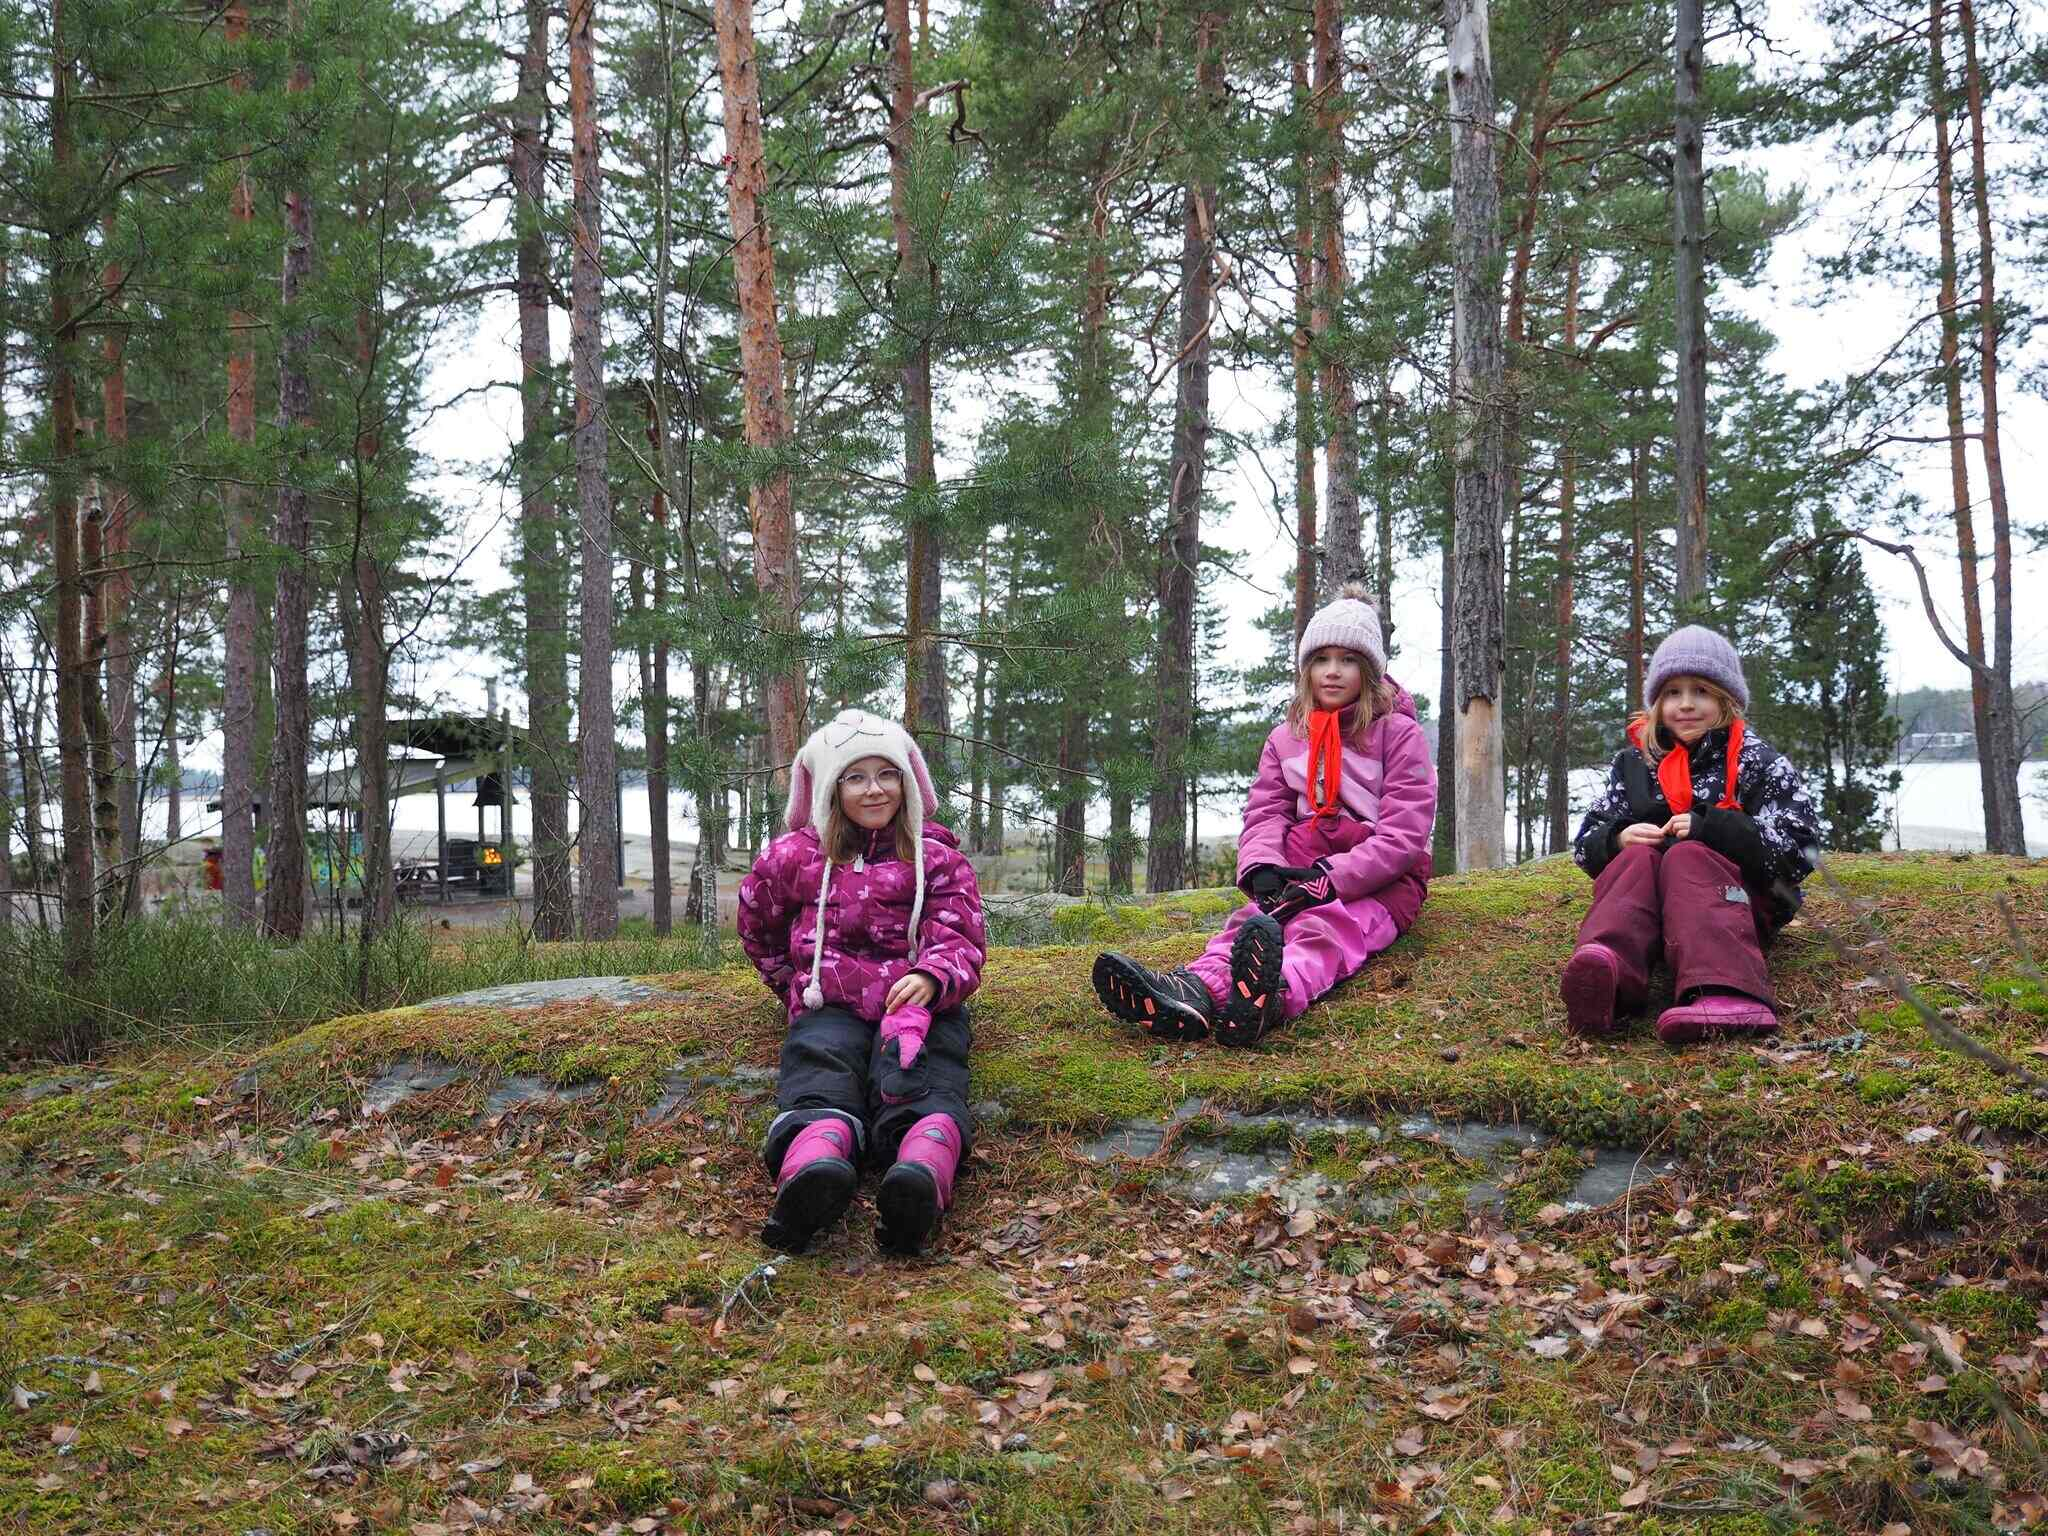
\includegraphics[width=\linewidth,trim={0 0.9cm 0 0.7cm},clip]{assets/pikkujoulu1}


\clearpage
\noindent Lippukuntaretkeltä (29.11.--1.12.) löytyi kirjoituskone, jolla kaikilla oli vapaus
kirjoittaa pari sanaa Tassuun. Tässä on tulos:

\vspace*{1.5cm}
\noindent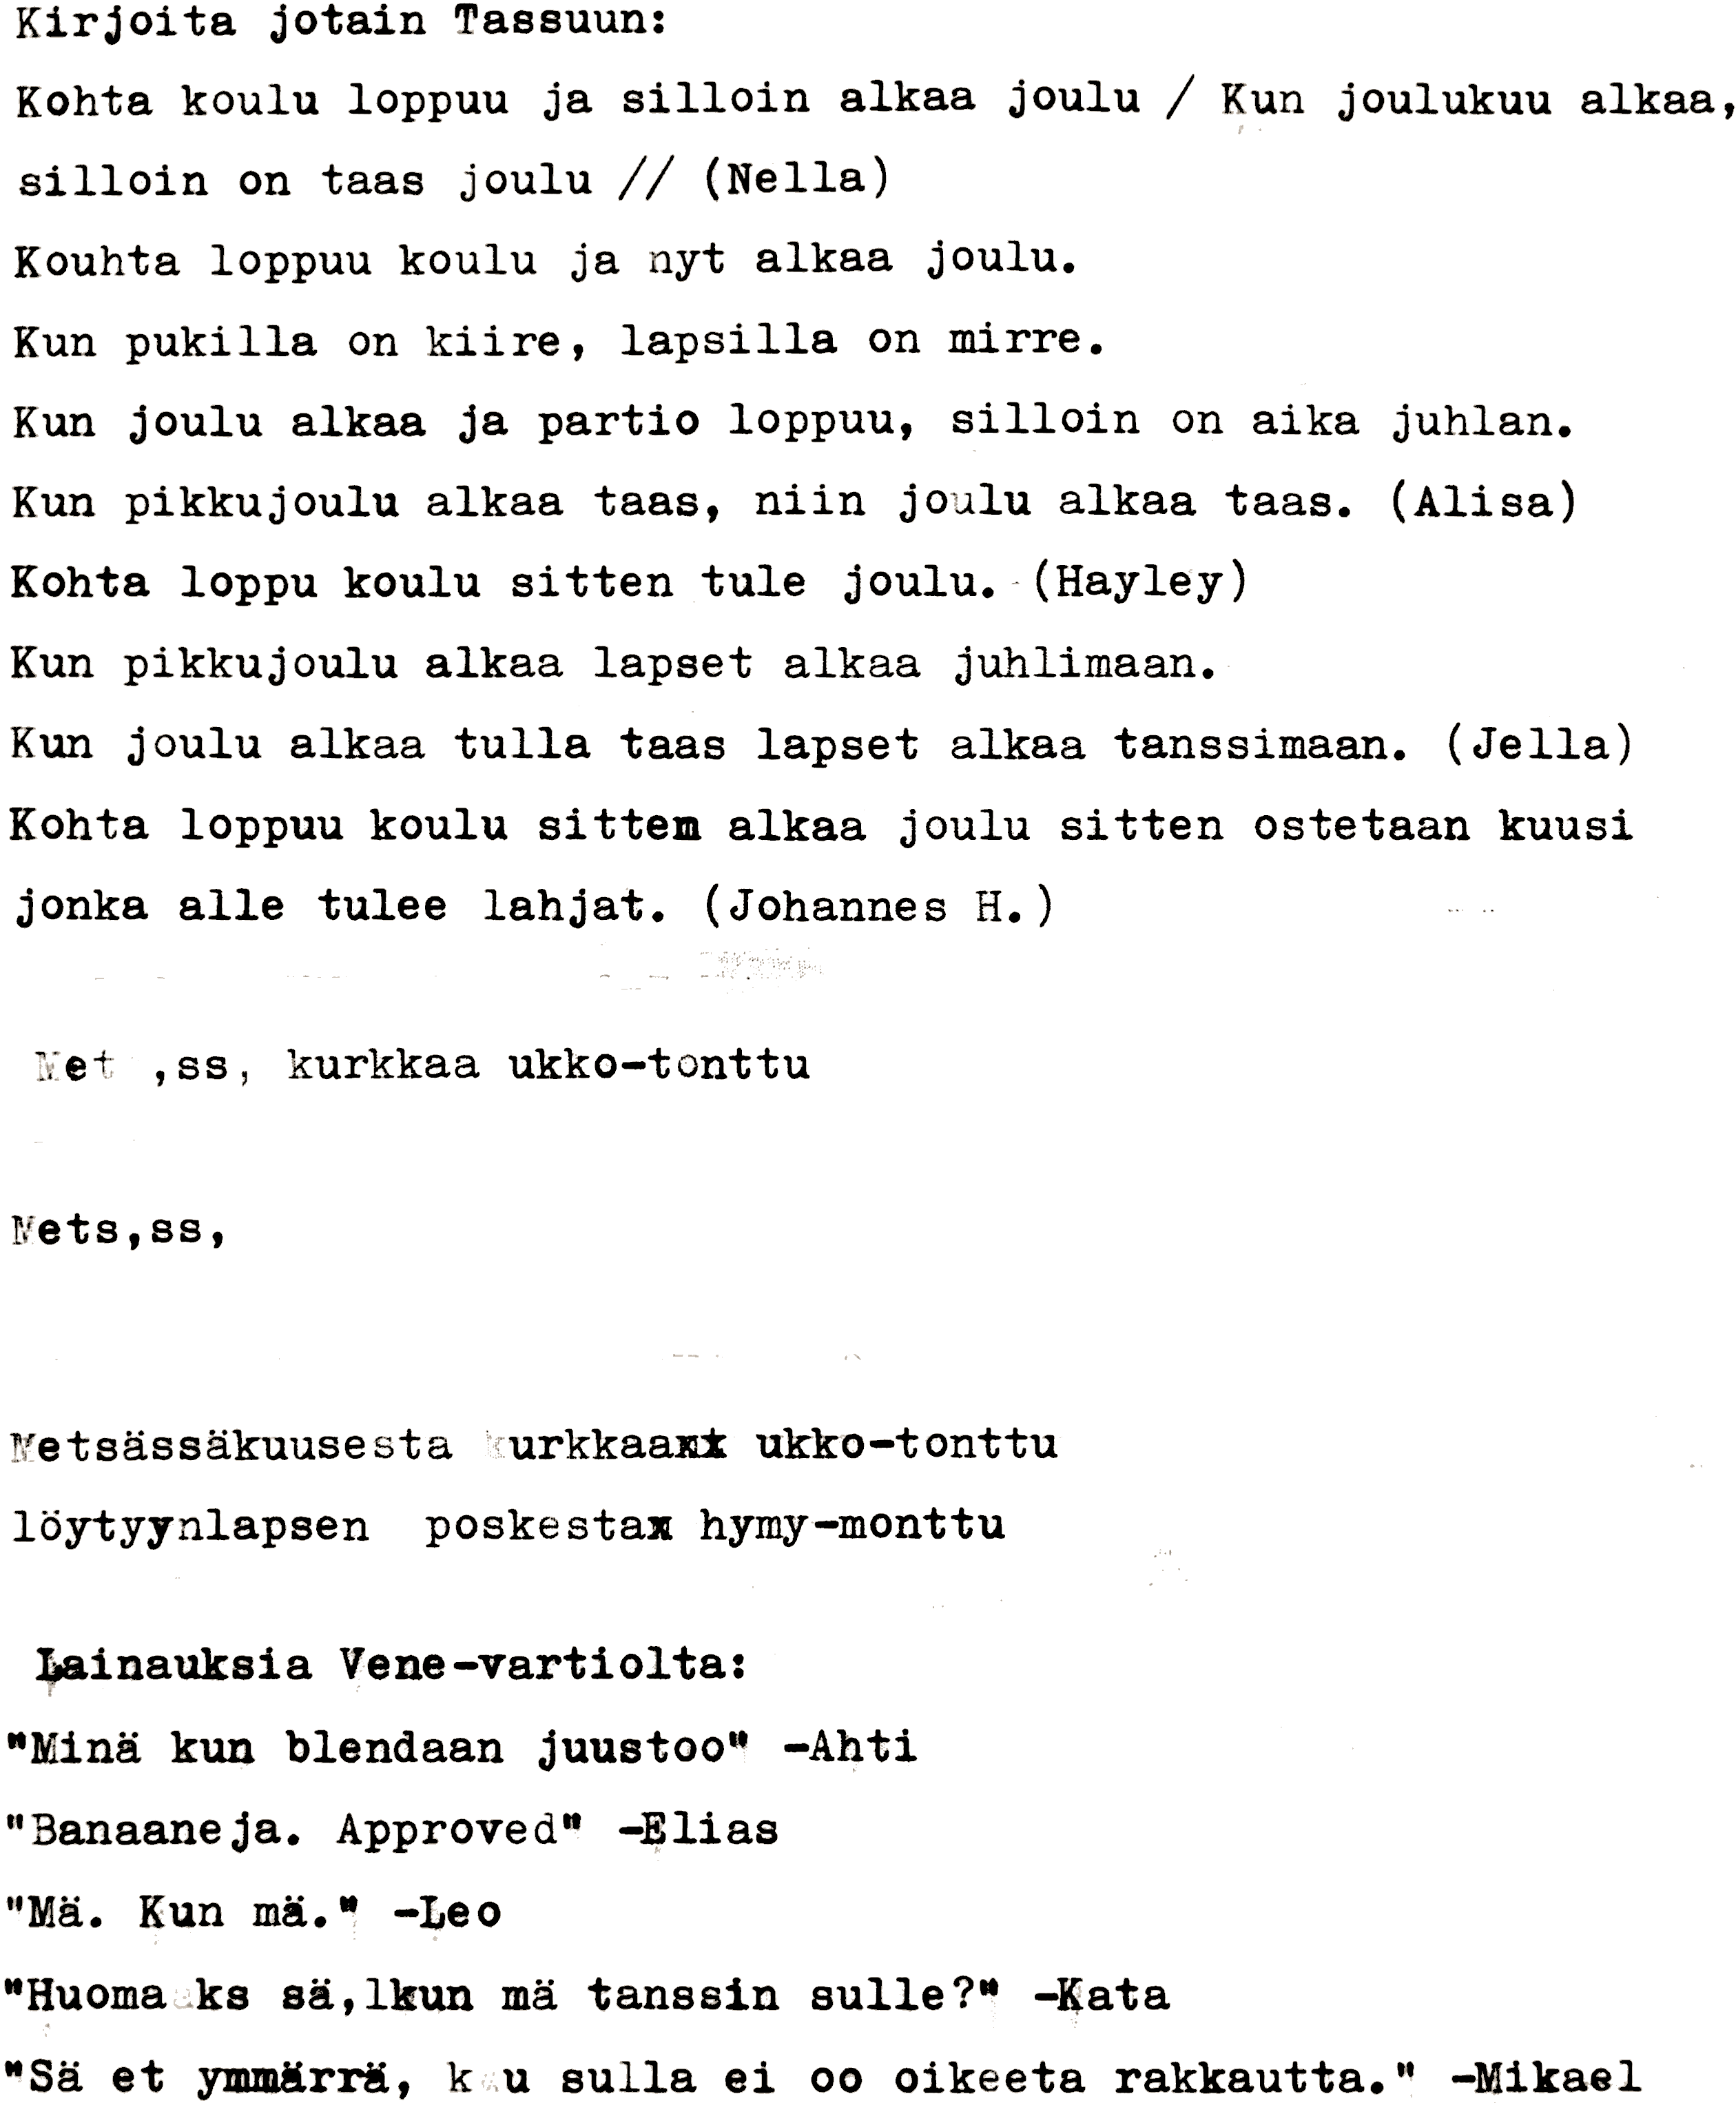
\includegraphics[width=\linewidth]{assets/pikkujoulu2}
